\documentclass[review]{elsarticle}

\usepackage{hyperref}
\usepackage{mathtools}
\usepackage{amssymb} % for \lessgtr
\usepackage{graphicx}
\usepackage{subcaption}
\usepackage{CJKutf8}
\usepackage[bottom]{footmisc}
\usepackage{siunitx}

\DeclarePairedDelimiter\set\{\}

\journal{産業応用工学会論文誌%(The Japanese Journal of the Institute of Industrial Applications Engineers)
}

\bibliographystyle{elsarticle-num}

%%%%%%%%%%%%%%%%%%%%%%%

\begin{document}

\begin{CJK}{UTF8}{min}

\begin{frontmatter}

\title{訪日中国人観光客のオンラインホテルレビューの感情分析と評価点の関係性分析 \\ Relation Analysis between Hotel Review Rating Scores and Sentiment Analysis of Reviews by Chinese Tourists Visiting Japan}

%% or include affiliations in footnotes:
\author[gidai]{Elisa Claire Alem\'an Carre\'on
\corref{mycorrespondingauthor}}
\ead{s153400@stn.nagaokaut.ac.jp}

\author[gidai]{Hirofumi Nonaka}
\ead{nonaka@kjs.nagaokaut.ac.jp}

\author[nagasaki]{Toru Hiraoka}
\ead{hiraoka@sun.ac.jp}

\address[gidai]{Nagaoka University of Technology, Nagaoka, Japan}
\address[nagasaki]{University of Nagasaki, Nagasaki, Japan}

\cortext[mycorrespondingauthor]{Corresponding author}

\begin{abstract}

In current times, the importance of online hotel review sites has become more and more apparent. Users of these sites reference of reviews strongly influences their purchase behavior and as such, reviews are important to companies and researchers alike. The majority of review sites offer both text reviews and numerical hotel ratings, and both information sources are widely used by researchers as a representation of a customer's sentiment and opinion. However, an opinion is a difficult concept to measure, and as such, depending on the relation these two sources have, it would be apparent whether or not it is safe to consider them equally in research. In this study we utilize an entropy-based Support Vector Machine to classify positive and negative sentiments in hotel reviews from the site \textit{Ctrip}, then calculating the ratio of positive and negative sentiment in each review and examine their correlation with said review's rating score using Spearman and Kendall Correlation coefficients and Maximal Information Coefficient (MIC).


\end{abstract}

\begin{keyword}

感情分析\sep 観光\sep SVM\sep 機械学習\sep Entropy

\end{keyword}

\end{frontmatter}

\section{はじめに}\label{intro}

訪日中国人観光客が増加する中,ホテル産業においては宿 泊客のニーズを分析するための市場調査を行うことが重要となっている。このような中で,アンケートやヒアリングなどでのニーズ把握が市場調査の中心になっている。しかしながら,このようなアンケートやヒアリングを用いた調査はコストやリアルタイム性の点で問題があった。一方で,インターネットの普及に伴い,オンラインレビューを通じた口コミが数多く存在する。ユーザが他人の意見を参考にし,購入行動を行うなどの影響がある\cite[][]{VERMEULEN2009123, SPARKS20111310}ため,産業界においても活発に利用されている。多くのオンラインレビューサイトにおけるユーザの評価は大きく,テキスト情報としてのコメント本文と数値で表現される評価点に分かれる。評価点については,構造化された数値情報であり解析に使うことが容易であるため,ユーザの商品・サービスに関する評価指標として利用されて いる\cite[][]{XIE20141, BULCHANDGIDUMAL201344, ZHOU20141}。一方,自然言語処理に基づいたコメント本文の分析も行われている。例えば,情報理論を利用して口コミの感情分析を行う研究\cite[][]{AMPLAYO201754}や感情分析に基づいて商品の売り上げの 予測\cite[][]{FAN201790}やランキング\cite[][]{LIU2017149}を行うなどの研究が行われている。

顧客動向分析においては,何を分析指標として使用するか は極めて重要な観点となる。前述の通り,先行研究では感情 分析のみ\cite[][]{AMPLAYO201754,LIU2017149},もしくは,評価点のみ\cite[][]{XIE20141, BULCHANDGIDUMAL201344, ZHOU20141}を使用して顧客動 向を解析した研究が多数ある。このため,これら評価点とコ メントの感情評価の関係性を検討する必要がある。仮に,評価点と文書の感情評価の関係性が高いとすれば,数値情報に基づく解析が容易な評価点のみを利用することや,数値情報を教師データに使用することでテキスト情報に基づいた感情 分析の学習にも役立つなどメリットは大きい。一方で関連性が低い場合には,評価点とテキスト情報を併用して総合的にレビューを評価する必要がある。あるいは,よりユーザの感情・意見が反映されている方法を選別して評価指標とする必要がある。このように,評価点とコメント本文の感情分析の関係性を調べることはレビューの分析にあたって極めて重要となる。

そこで,本研究では,評価点とコメント本文の感情分析の 関係性について調査を行った。本研究では,まず,中国人観光客向けのオンラインホテルレビューサイト\textit{Ctrip}から日本のホテルについて書かれた大量のレビュー文書とその評価点の収集を行った。次に,本研究者らが開発したエントロピーをベースとする素性選択手法を用いてSVMで学習し,Positiveな感情を表す文書とNegativeな感情を表す文書の分類を行った。この感情分類に特徴的な素性ベクトルをエントロピーベースでのキーワード抽出により構築したため,統計量に基づいた言語に依存しない手法を利用して分類を行った。さらに各レビューの各文の感情分類に基づき,感情の数値化をするために満足を表す文の比率と不満を表す比率を算出した。最後に評価点とレビューの感情評価の相互関係性を,スピアマンの順位相関係数,ケンドールの順位相関係数MICより分析した。以下,詳細に説明する。


\section{従来研究}\label{lit_rev}

従来のレビュー解析においては商品レビューを対象としたものが主流である。例としてはWord Cloudを適用し消費者が多く使われる単語の抽出を行なった研究\cite[][]{hargreaves2015}や,HowNetという感情辞書を利用して商品のレビューの感情分析を行なった上でマーケット調査に適用した研究\cite[][]{zhang2011feature}がある。一方でホテルのオンラインレビューの影響を定量的に評価しているものとしては,ホテルオンラインレビューが顧客の意欲に特徴的な影響を与えられることを証明した研究がある\cite[][]{VERMEULEN2009123}。他に,売り上げと評価されるレビューのテキスト情報との関係性を示した研究がある\cite[][]{basuroy2003}。以上の研究では,評価点は考慮したものではなく,評価点とテキスト情報の関係性に着目したものではなかった。

\section{手法}\label{methodology}

\subsection{前処理}\label{preprocessing}

クローリングの段階でCtripの各ホテルの特徴としてURLの構造がID番号で決められていることを利用し,自動的に一つ一つのホテルのページを読み込むことができる。次にスクレイピングを行い,HTMLの特徴を利用して各レビューの文書,ID,評価点など取得し,データベースに保存した。レビューに対しては形態素解析も行った。中国語の形態素解析のツールとしては,スタンフォード大学のThe Stanford NLP Groupが提供しているStanford Word Segmenter\cite[][]{chang2008}を利用した。

\subsection{感情分析}\label{sentiment_analysis}

感情分析を行うためにオンラインホテルレビューの収集したデータから標本を抽出し、中国人の研究生3人の協力をいただき、各レビューの各文は満足を表すか、不満店を表現しているかによってタグ付けのPositiveとNegativeの手動分類を行い、教師データを作成した。それから標本のレビューに含まれる語と感情分類タグをSVMに学習させ、母集団となる全データの感情分類を行った。SVMによった感情分類に特徴的な素性ベクトルを後述のエントロピーベースでのキーワード抽出により構築した。以下,その詳細を説明する。

\subsubsection{エントロピーベースキーワード抽出}\label{entropy}

本研究では統計的にもっとも感情と関連しているキーワードを抽出するためにシャノンのエントロピー\cite[][]{shannon1948}を利用した。情報理論の分野では,シャノンのエントロピーは信号の情報量の期待値である。すなわち,ある事象の予測不可能性を表す。この概念に基づいて,事象の確率分布の偏在性を表すことができる。例えば,コーパス内のほとんどの文書に含まれる語がどの特定の文書に現れるかの予測は困難になり,その語のエントロピーは高くなる。逆に,特定の文書によく現れ,他の文書にほぼ含まれない大きな文書偏在性を持つ単語を考えると,どの文書に含まれるかという予測の曖昧さは減少し,エントロピーは0に近づく。Fig.\ref{fig:entropygraphs}にこの概念を示す。

以上のエントロピーの物理的意味に基づくと,Positiveに関連するキーワードはPositiveが出現する文書セットでエントロピーが大きく,Negativeが出現する文書セットではエントロピーは小さいことが言える。これはNegativeに関連するキーワードでも同様である。そこで本研究ではエントロピーを利用した感情分類における素性選択を行う。まず,レビューに2値の感情分類をタグ付けし,各ワード\(j\) が各文書\(i\)に含まれる回数を,Positiveな文書の場合に\(N_{ijP}\),Negativeな文書の場合に\(N_{ijN}\)を算出する。次に以下に示す式を利用し,各ワードのPositiveとNegativeの文書に含まれる確率,\(P_{ijP}\) (\ref{eq:PijP})と\(P_{ijN}\) (\ref{eq:PijN})を算出する。

\begin{figure}[h]
    \centering
    \begin{subfigure}[b]{0.4\linewidth}
        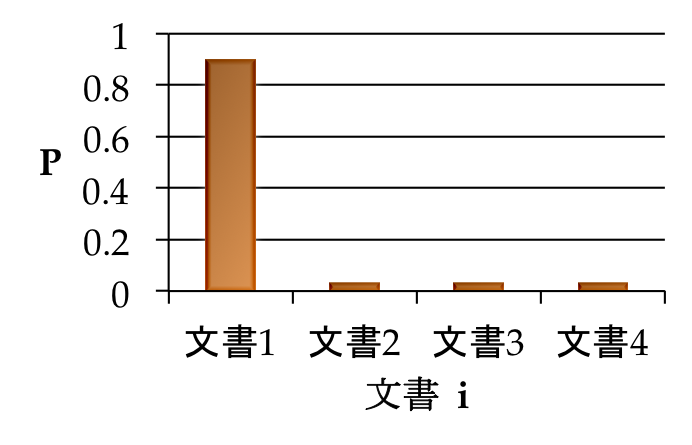
\includegraphics[width=\linewidth]{entropyzero_jp.png}
        \caption{エントロピーが0に近い}
    \end{subfigure}
    \begin{subfigure}[b]{0.4\linewidth}
        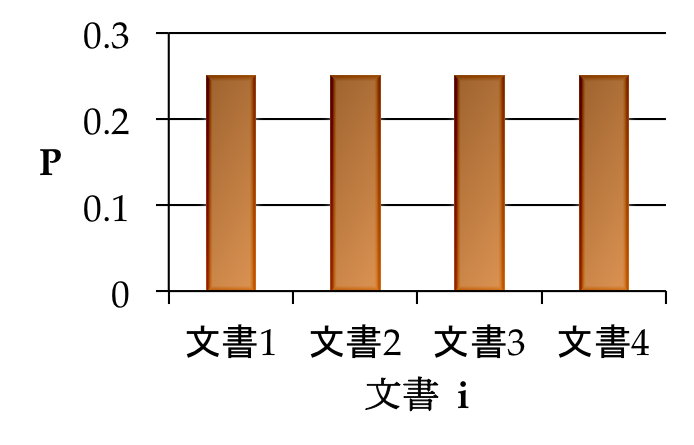
\includegraphics[width=\linewidth]{entropyhigh_jp.png}
        \caption{エントロピーが高い}
    \end{subfigure}
\caption{ワード\(j\)が文書\(i\)に含まれる確率Pを棒グラフで表示}
\label{fig:entropygraphs}
\end{figure}



\begin{equation}\label{eq:PijP}
P_{ijP} = \frac{N_{ijP}}{\sum_{i=1}^M N_{ijP}}
\end{equation}

\begin{equation}\label{eq:PijN}
P_{ijN} = \frac{N_{ijN}}{\sum_{i=1}^M N_{ijN}}
\end{equation}

以上の値を次の式に代入し,各ワード\(j\)のPositiveに関するエントロピー\(H_{Pj}\) (\ref{eq:Hpj}),各ワード\(j\)のNegativeに関するエントロピー\(H_{Nj}\) (\ref{eq:Hnj})を算出した。ただし,確率が0となる場合については式(\ref{eq:lim_Hpj})と(\ref{eq:lim_Hnj})に示す極限を利用して(\ref{eq:Hpj})と(\ref{eq:Hnj})の和に代入する。

\begin{equation}\label{eq:Hpj}
H_{Pj} = - \sum_{i=1}^M [P_{ijP}\log_2 P_{ijP}]
\end{equation}

\begin{equation}\label{eq:lim_Hpj}
\lim_{P_{ijP}\to0+} P_{ijP}\log_2 P_{ijP} = 0
\end{equation}

\begin{equation}\label{eq:Hnj}
H_{Nj} = - \sum_{i=1}^M [P_{ijN}\log_2 P_{ijN}]
\end{equation}

\begin{equation}\label{eq:lim_Hnj}
\lim_{P_{ijN}\to0+} P_{ijN}\log_2 P_{ijN} = 0
\end{equation}

各語の感情分類毎のエントロピーを算出した後,\(\alpha\) の調整を行った。\(\alpha\)は評価データのF値がもっとも高くなるものを選択する。最適な\(\alpha\)のもとで以下の(\ref{eq:entropy_pos}),(\ref{eq:entropy_neg})を計算し,(\ref{eq:entropy_pos})を満たす語をPositiveのキーワード,(\ref{eq:entropy_neg})を満たす語をNegativeのキーワードと分類した。これを素性としてSVM\cite[][]{cortes1995}による学習を行った。評価はk-fold cross validationを用いてF1\cite[][]{powers2011}により行なった。

\begin{equation}\label{eq:entropy_pos}
H_{Pj} > \alpha H_{Nj}
\end{equation}

\begin{equation}\label{eq:entropy_neg}
H_{Nj} > \alpha' H_{Pj}
\end{equation}

\subsection{相関分析}\label{correlation}

各レビューに含まれるポシティブとして判定された文を全体で割った率 x が評価点 y の関連性を測るために次に述べる手法を実験的に利用した。

\subsubsection{ピアソン相関係数 \(r\)}\label{correl_pearson}

各レビューに含まれるポシティブとして判定された文\(i_P\)を全体の文の数\(i_T\)で割った率\(x\)が評価点\(y\)の関連性を測るためその一つとしてピアソンの相関係数\(r\)(\ref{eq:pearson_r})を利用した。以下に式を示す。式(\ref{eq:pearson_r})に式(\ref{eq:pos_neg_ratio})の値を代入する。ネガティブ率を計算する際には式(\ref{eq:pos_neg_ratio})にネガティブと判定された文\(i_N\)を代入する。

\begin{equation}\label{eq:pos_neg_ratio}
x = \frac{i_P}{i_T}
\end{equation}

\begin{equation}\label{eq:pearson_r}
r = \frac{{}\sum_{i=1}^{M} (x_i - \overline{x})(y_i - \overline{y})}
{\sqrt{\sum_{i=1}^{M} (x_i - \overline{x})^2(y_i - \overline{y})^2}}
\end{equation}

\subsubsection{スピアマンの順位相関係数 \(\rho\)}\label{correl_spearman}

各レビューに含まれるポシティブとして判定された文 iP を全体の文の数\(i_T\)で割った率\(x\)が評価点\(y\)の関連性を測るため,評価点が順位を表すものだと考える上で順位変数にピアソンの相関係数に基づいたスピアマンの順位相関係数\(\rho\)(\ref{eq:spearman_rho})を利用した。以下に式を示す。式(\ref{eq:spearman_rho})に式(\ref{eq:pos_neg_ratio})の値を代入する。

\begin{equation}\label{eq:spearman_rho}
r_s = \rho_{rg_X,rg_Y} = \frac{cov(rg_X,rg_Y)}{\sigma_{rg_X} \sigma_{rg_Y}}
\end{equation}

\subsubsection{ケンダルの順位相関係数\(\tau\)}\label{correl_kendall}

スピアマンの順位相関係数のように,ケンダルの順位相関係数は順位を表す値の関係性を調べるために用いるものである。以下に式(\ref{eq:kendall_tau})を示す。ただし,式(\ref{eq:kendall_tau})に式(\ref{eq:kendall_L})と式(\ref{eq:kendall_K})を代入する。それぞれに式(\ref{eq:pos_neg_ratio})を代入する。


\begin{equation}\label{eq:kendall_tau}
\tau = (K-L)/\dbinom{n}{2}
\end{equation}

\begin{equation}\label{eq:kendall_L}
L = \# \set[\Big]{\{i,j\} \in \binom{[n]}{2} \mid \neg (x_i \lessgtr x_j, y_i \lessgtr y_j ) }
\end{equation}

\begin{equation}\label{eq:kendall_K}
K = \# \set[\Big]{\{i,j\} \in \binom{[n]}{2} \mid (x_i \lessgtr x_j, y_i \lessgtr y_j ) }
\end{equation}

\subsubsection{MIC}\label{mic}

ピアソンの相関係数は線形の関係性のみ抽出できる。一方で,非線形性も含めた二変数間の関連性を分析する手法としてMIC(Maximal Information Coefficient)がある\cite[][]{Reshef2011}。関連性を分析したい二変数を確率変数と捉えて,その相互情報量に基づき非線形性も含めた変数間の関連性を分析するための指標である。MICとピアソンの係数を比較する複数の例をFig.\ref{fig:mic}に示す。ピアソンの係数は線型的な関係性で0から1までの値となり、傾きの方向によって正の値か負の値か決定される。一方で、MICの場合には非線形的な関係性でも、関係性がある限り0から1の値を利用して総合関係を表すことはFig.\ref{fig:mic}の各例に比較が示される。

MICの算出手順について述べておく。まず,分析対象である変数\(X\),\(Y\)に対して,二変数を座標空間上にプロットしたあとで,\(a*b\)(\(X\)方向に\(a\)分割,\(Y\)方向に\(b\)分割)のセルへ分割を行う。その上で二変数それぞれについて,各セルに所属するサンプル点の数を全サンプル数で除すことでセルの存在確率を算出することができる。すなわち,\(X\),\(Y\)をセルにおける存在確率をベースとした確率変数と捉える。これにより\(X\),\(Y\)に関する相互情報量を計算することができる。

\begin{figure}[h]
\centering
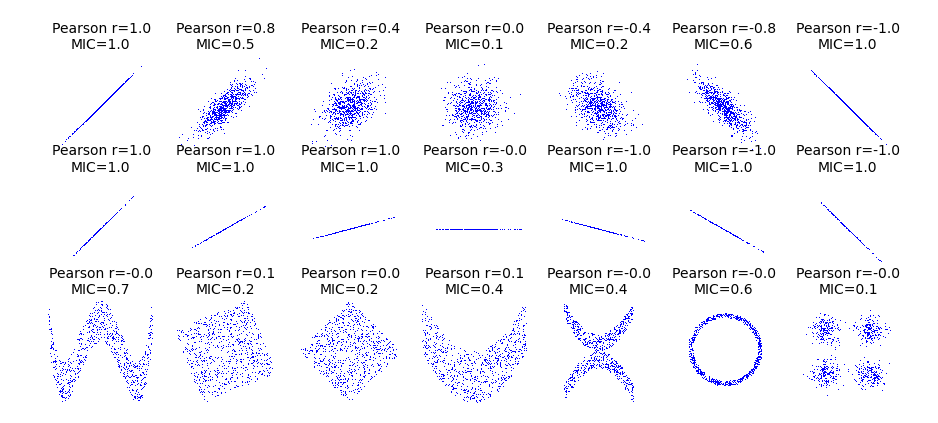
\includegraphics[width=20em]{MIC_pearson_relationships.png}
\caption{minepyのMICとピアソンの\(r\)を様々な場合での比較}
\label{fig:mic}
\end{figure}

このとき,もとの二変数が線形の関係に限らず非線形の関係にある場合でも,確率変数間の依存性は強くなるため,相互情報量は大きな値をとる。よってピアソンの相関係数と異なり非線形の関係性を抽出することが可能となる。なお,MICでは,各セルの幅と長さは非等間隔とするため,分割方法は無数に存在する(なお,セルには,最大解像度が存在するものとする)。非線形性の抽出という目的のためにはなるべく,相互情報量を最大化するような分割グリッドを見つける必要がある。MICでは,今,\(X\)を任意の\(a\)個,\(Y\)を任意の\(b\)個に分割したと仮定する。このとき総当たりで\(a*b\)の分割における相互情報量を最大化する分割を見出す。相互情報量の式(15)を以下に示す。

\begin{equation}
I(X;Y) = \int_{Y}{\int_{X}{p(x,y)\log(\frac{p(x,y)}{p(x)p(y)})}\,dx}\,dy
\end{equation}

本研究ではPythonのライブラリminepy\cite[][]{Albanese2012}を利用してMICを算出した。以下にピアソンの相関係数とMICを比較するFig.\ref{fig:mic}をminepyのAPIのサイトから取得した。

\section{実験結果}\label{results}

以前に述べた手法を利用し,具体的に本研究で行われたことを以下に述べる。

\subsection{前処理}\label{res_preprocessing}

まず,\textit{Ctrip}より,2016年5月から2016年9月までの154万1424件のHTMLファイルを収集した。154万1424個HTMLファイルのうち,5938件の日本に存在するホテルのデータを収集した。その中に存在した 4万4912件のレビューのコメント本文をスクレイピングした。これらについて文単位に分割した28万6109文を解析対象とする。また,あわせてレビューの評価点も収集した。

\subsection{感情分類の評価実験}\label{res_sentiment_analysis}

教師データを作成するためには全データからレビューの標本をランダムに抽出し、満足か不満を表すことにより文ごとに分割し、159文のタグ付け作業を手動で行い、教師データとなる文からエントロピーの計算を行った。

教師データに関してエントロピーを計算した後,最適な\(\alpha\)の値を求めるため1.0から3.75まで,0.25の刻み幅で評価し,最大のF1値を持つ素性を選択した。SVMでの学習後,評価データに対して5-Fold Cross Validation(\(k = 5\))の結果,F1値が最大となった\(\alpha\)に基づきキーワードリストを選択した。さらに,両方のリストを組み合わせ,新たなリストを作成し,同様に5-Fold Cross Validation を行った。それらの評価結果をTable 1に示す。両方を組み合わせた素性が最もF1値が高くなり、F1は0.95の高い精度を持ったSVMで全データの分類を行った。Positiveなキーワードは例えば、「热情」、「景色」(それぞれ「人懐っこい」、「(良い)景色」を示す)で、Negativeな場合「价格」(高いため不満を示す)の例があった。

%table 1

%table 2

最適なモデルでの学習後,未知データに関して感情分析を行い,前述の「Positive率」と「Negative率」を算出した。これらの値は満足を表す文章と不満足を表現する文章の比率であるため、各文章の感情を表す数値的な係数として扱い、相関分析を行った。


\subsection{相関分析}\label{res_correls}

全データにある各レビューのPositive率とNegative率とそのレビューの評価点についてスピアマンの順位相関係数,ケンドールの順位相関係数,MICを利用して関連性分析を行った。その結果をTable 2で示す。

\section{考察}\label{discussion}

全ての指標において,Positive率,Negative率ともに評価点との関連性が非常に低いことを示した。

よって、コメント本文における感情分析の結果と評価点の関係性は低いことからユーザの意見をレビューより分析する際には,テキストの内容と数値的な評価点の双方についてそしてそれらの違いを検討することが重要である。

従来、この関係性は示されていないにも関わらず、満足度や感情評価の指標として評価点のみが使用されることは多くある。例えば、XieらとBulchand-Gidumalらの研究にはホテル全体の評価点を満足度の代理であると出張しており\cite[][]{XIE20141, BULCHANDGIDUMAL201344}、Zhouらは満足の要因を調査するために多変数分析を利用したが、従属変数は評価点であった\cite[][]{ZHOU20141}。
このような研究に対して、本研究の結果を踏まえて、評価点のみ、または、感情分析のみを観光客の満足度を測る指標として利用することは適切ではないことが示唆された。

\section{おわりに}\label{conclusion}

本研究ではオンラインホテルレビューのテキスト本文の感情分析の結果と評価点の関係性を調べた。感情分析に当たって分類性能が高い(F1 = 0.95) 手法を構築し,各口コミのPositiveと分類された文の比率とNegativeと分類された文の比率を算出した。関係性についてはスピアマンの順位相関係数,ケンドールの順位相関係数とMICを利用した。その結果,いずれも低い値を示した。よって、コメント本文の感情分析の結果と数値情報である評価点の関係性は低いことが明らかになった。よって、より全面的な評価が重要であると考察された。今後はこれらの結果を踏まえて、多言語の情報を利用した解析と比較をした上で感情分析の結果と評価点のどちらがよりユーザの意見を表現しているか調査を行い,レビューの総合的な分析手法の開発を進めていく。

\section*{謝辞}\label{acknowledgements}

中国語での教師データ作成等で支援をいただいた周良遠氏,エルデェンチチグ氏に感謝する。また、本論文は「財団法人日本建設情報総合センター」の支援で行なわれた。

\clearpage

\bibliography{jjiiae}

\end{CJK}

\end{document}